\documentclass[11pt,a4paper]{article}
\usepackage[T1]{fontenc}
\usepackage[utf8]{inputenc}
\usepackage{lmodern}
\usepackage[varqu,scaled=0.95]{zi4}
\usepackage[margin=2.3cm,headheight=14pt]{geometry}
\usepackage{microtype}
\usepackage{graphicx}
\usepackage{booktabs}
\usepackage{tabularx}
\usepackage{amsmath,amssymb}
\usepackage{float}
\usepackage{placeins}
\usepackage{needspace}
\usepackage{xcolor}
\usepackage[parfill]{parskip}
\usepackage{enumitem}
\usepackage{titlesec}
\usepackage{fancyhdr}
\usepackage[font=small,labelfont={bf,color=accent},skip=6pt]{caption}
\usepackage{listings}
\usepackage[most]{tcolorbox}
\usepackage[colorlinks=true,linkcolor=accent,citecolor=accent,urlcolor=accent]{hyperref}

% ---------------------------------------------------------------------
% Colours (methods match the figures)
\definecolor{accent}{HTML}{1F3A5F}
\definecolor{accentlight}{HTML}{EEF3F9}
\definecolor{rulegray}{HTML}{C9D3DF}
\definecolor{codebg}{HTML}{F8F9FB}
\definecolor{codekw}{HTML}{8A3FA0}
\definecolor{codecomment}{HTML}{6B7785}
\definecolor{mikj}{HTML}{EB6834}
\definecolor{mblocked}{HTML}{4A3AA7}
\definecolor{momp}{HTML}{2A78D6}

% ---------------------------------------------------------------------
% Headings
\titleformat{\section}{\Needspace{8\baselineskip}\Large\bfseries\color{accent}}{\thesection}{0.7em}{}
  [\vspace{-4pt}{\color{rulegray}\titlerule[0.8pt]}]
\titlespacing*{\section}{0pt}{18pt}{10pt}
\titleformat{\subsection}{\Needspace{7\baselineskip}\large\bfseries\color{accent}}{\thesubsection}{0.6em}{}
\titlespacing*{\subsection}{0pt}{14pt}{6pt}

% A concept heading on its own line, with space above, inside a section
\newcommand{\concept}[1]{\par\addvspace{8pt}\Needspace{5\baselineskip}%
  \noindent{\color{accent}\bfseries\boldmath #1}\par\nopagebreak\vspace{2pt}}

% Page style
\pagestyle{fancy}
\fancyhf{}
\fancyhead[L]{\small\color{codecomment}Assignment 3 \textperiodcentered{} Parallel matrix multiplication}
\fancyhead[R]{\small\color{codecomment}\AuthorName}
\fancyfoot[C]{\small\thepage}
\renewcommand{\headrulewidth}{0.4pt}
\renewcommand{\headrule}{{\color{rulegray}\hrule height\headrulewidth}}

% Lists
\setlist{itemsep=3pt,parsep=0pt,topsep=4pt}

% Floats: let large figures and tables share pages with text instead of leaving gaps
\renewcommand{\topfraction}{0.85}
\renewcommand{\bottomfraction}{0.6}
\renewcommand{\textfraction}{0.1}
\renewcommand{\floatpagefraction}{0.8}
\setcounter{topnumber}{3}
\setcounter{totalnumber}{4}

% ---------------------------------------------------------------------
% Boxes
\newtcolorbox{infobox}[1][]{enhanced,breakable,colback=accentlight,colframe=accent,
  boxrule=0pt,leftrule=3pt,arc=0pt,left=10pt,right=10pt,top=6pt,bottom=6pt,
  before upper={\setlength{\parskip}{5pt}},#1}
\newtcolorbox{titledbox}[1]{enhanced,breakable,colback=accentlight,colframe=accent,
  boxrule=0.6pt,arc=2pt,left=10pt,right=10pt,top=6pt,bottom=6pt,
  title={\bfseries #1},fonttitle=\normalsize,coltitle=white,
  before upper={\setlength{\parskip}{5pt}}}

% Code listings
\lstdefinestyle{kernel}{
  basicstyle=\ttfamily\small,
  keywordstyle=\color{codekw}\bfseries,
  commentstyle=\color{codecomment}\itshape,
  stringstyle=\color{codecomment},
  numbers=left, numberstyle=\scriptsize\color{codecomment}, numbersep=8pt,
  showstringspaces=false, columns=fullflexible, keepspaces=true,
  aboveskip=0pt, belowskip=0pt, xleftmargin=14pt
}
\newtcblisting{codebox}[3]{enhanced,breakable,listing only,
  listing options={style=kernel,language=#1},
  colback=codebg,colframe=#3,boxrule=0.6pt,leftrule=3pt,arc=2pt,
  left=4pt,right=6pt,top=4pt,bottom=4pt,
  title={\ttfamily\small #2},coltitle=black,colbacktitle=#3!12,
  fonttitle=\bfseries,toptitle=1pt,bottomtitle=1pt}

% Tables
\renewcommand{\arraystretch}{1.12}

% ---------------------------------------------------------------------
% Generated by scripts/analyze.py -- do not edit by hand.
\newcommand{\BlockedTimeTable}{
\begin{tabular}{r r r r r r r r r r r }\toprule
& Sequential & \multicolumn{9}{c}{OpenMP, $p$ threads} \\\cmidrule(lr){3-11}
$n$ & blocked\_seq & 1 & 2 & 4 & 6 & 8 & 12 & 16 & 24 & 32 \\\midrule
256 & 3.4 ms {\scriptsize(15)} & 2.9 ms {\scriptsize(11)} & 2.1 ms {\scriptsize(17)} & 986 $\mu$s {\scriptsize(3)} & 1.4 ms {\scriptsize(14)} & 1.8 ms {\scriptsize(18)} & 13.7 ms {\scriptsize(20)} & 2.6 ms {\scriptsize(40)} & 2.4 ms {\scriptsize(23)} & 4.1 ms {\scriptsize(4)} \\
512 & 25.9 ms {\scriptsize(10)} & 28.4 ms {\scriptsize(17)} & 22.5 ms {\scriptsize(16)} & 13.4 ms {\scriptsize(16)} & 11.7 ms {\scriptsize(2)} & 7.7 ms {\scriptsize(123)} & 5.5 ms {\scriptsize(184)} & 7.4 ms {\scriptsize(21)} & 6.6 ms {\scriptsize(8)} & 6.5 ms {\scriptsize(100)} \\
1024 & 197.4 ms {\scriptsize(6)} & 194.3 ms {\scriptsize(7)} & 106.2 ms {\scriptsize(8)} & 64.6 ms {\scriptsize(16)} & 48.3 ms {\scriptsize(7)} & 92.4 ms {\scriptsize(128)} & 104.8 ms {\scriptsize(17)} & 74.9 ms {\scriptsize(23)} & 74.7 ms {\scriptsize(9)} & 84.9 ms {\scriptsize(4)} \\
2048 & 1.61 s {\scriptsize(1)} & 1.59 s {\scriptsize(1)} & 887.9 ms {\scriptsize(4)} & 534.8 ms {\scriptsize(1)} & 384.2 ms {\scriptsize(1)} & 734.5 ms {\scriptsize(45)} & 519.4 ms {\scriptsize(54)} & 477.3 ms {\scriptsize(48)} & 554.6 ms {\scriptsize(42)} & 643.7 ms {\scriptsize(24)} \\
3072 & 5.41 s {\scriptsize(1)} & 5.36 s {\scriptsize(0)} & 3.08 s {\scriptsize(4)} & 1.62 s {\scriptsize(3)} & 1.70 s {\scriptsize(2)} & 1.52 s {\scriptsize(2)} & 1.81 s {\scriptsize(8)} & 1.72 s {\scriptsize(12)} & 1.61 s {\scriptsize(5)} & 1.63 s {\scriptsize(9)} \\
4096 & 12.86 s {\scriptsize(0)} & 12.76 s {\scriptsize(1)} & 7.91 s {\scriptsize(7)} & 4.13 s {\scriptsize(11)} & 4.13 s {\scriptsize(3)} & 3.81 s {\scriptsize(6)} & 4.29 s {\scriptsize(2)} & 3.88 s {\scriptsize(8)} & 4.10 s {\scriptsize(7)} & 3.67 s {\scriptsize(16)} \\
6144 & 44.39 s {\scriptsize(0)} & 44.33 s {\scriptsize(0)} & 25.85 s {\scriptsize(1)} & 15.88 s {\scriptsize(1)} & 12.42 s {\scriptsize(1)} & 11.34 s {\scriptsize(5)} & 13.41 s {\scriptsize(4)} & 13.25 s {\scriptsize(21)} & 13.16 s {\scriptsize(21)} & 12.31 s {\scriptsize(16)} \\
\bottomrule\end{tabular}}
\newcommand{\IkjTimeTable}{
\begin{tabular}{r r r r r r r r r r r }\toprule
& Sequential & \multicolumn{9}{c}{OpenMP, $p$ threads} \\\cmidrule(lr){3-11}
$n$ & ikj\_seq & 1 & 2 & 4 & 6 & 8 & 12 & 16 & 24 & 32 \\\midrule
256 & 3.2 ms {\scriptsize(2)} & 3.1 ms {\scriptsize(5)} & 2.5 ms {\scriptsize(6)} & 1.0 ms {\scriptsize(23)} & 7.7 ms {\scriptsize(59)} & 1.4 ms {\scriptsize(3)} & 1.4 ms {\scriptsize(24)} & 1.6 ms {\scriptsize(46)} & 4.3 ms {\scriptsize(97)} & 1.6 ms {\scriptsize(104)} \\
512 & 23.5 ms {\scriptsize(4)} & 23.3 ms {\scriptsize(2)} & 12.8 ms {\scriptsize(4)} & 12.1 ms {\scriptsize(364)} & 83.9 ms {\scriptsize(127)} & 8.9 ms {\scriptsize(2)} & 10.1 ms {\scriptsize(8)} & 9.4 ms {\scriptsize(8)} & 7.8 ms {\scriptsize(6)} & 8.7 ms {\scriptsize(16)} \\
1024 & 252.5 ms {\scriptsize(18)} & 211.3 ms {\scriptsize(4)} & 134.6 ms {\scriptsize(3)} & 610.4 ms {\scriptsize(22)} & 86.6 ms {\scriptsize(10)} & 86.3 ms {\scriptsize(11)} & 91.2 ms {\scriptsize(6)} & 83.1 ms {\scriptsize(22)} & 79.4 ms {\scriptsize(11)} & 63.5 ms {\scriptsize(53)} \\
2048 & 3.34 s {\scriptsize(0)} & 3.33 s {\scriptsize(1)} & 2.03 s {\scriptsize(1)} & 1.25 s {\scriptsize(2)} & 929.2 ms {\scriptsize(4)} & 802.0 ms {\scriptsize(2)} & 679.6 ms {\scriptsize(8)} & 601.1 ms {\scriptsize(35)} & 656.0 ms {\scriptsize(19)} & 749.2 ms {\scriptsize(14)} \\
3072 & 11.36 s {\scriptsize(0)} & 11.41 s {\scriptsize(0)} & 6.96 s {\scriptsize(1)} & 3.61 s {\scriptsize(2)} & 3.11 s {\scriptsize(1)} & 2.81 s {\scriptsize(8)} & 2.53 s {\scriptsize(4)} & 2.58 s {\scriptsize(9)} & 3.27 s {\scriptsize(1)} & 3.29 s {\scriptsize(12)} \\
4096 & 27.61 s {\scriptsize(0)} & 27.49 s {\scriptsize(0)} & 16.76 s {\scriptsize(1)} & 8.90 s {\scriptsize(3)} & 6.32 s {\scriptsize(14)} & 5.60 s {\scriptsize(1)} & 6.19 s {\scriptsize(2)} & 5.68 s {\scriptsize(5)} & 9.63 s {\scriptsize(34)} & 11.35 s {\scriptsize(7)} \\
\bottomrule\end{tabular}}
\newcommand{\BlockedSpeedupTable}{
\begin{tabular}{r r r r r r r r r r }\toprule
$n$ & $p=1$ & $p=2$ & $p=4$ & $p=6$ & $p=8$ & $p=12$ & $p=16$ & $p=24$ & $p=32$ \\\midrule
256 & 1.15 {\scriptsize\color{codecomment}115\%} & 1.60 {\scriptsize\color{codecomment}80\%} & 3.42 {\scriptsize\color{codecomment}86\%} & 2.37 {\scriptsize\color{codecomment}40\%} & 1.89 {\scriptsize\color{codecomment}24\%} & 0.25 {\scriptsize\color{codecomment}2\%} & 1.30 {\scriptsize\color{codecomment}8\%} & 1.43 {\scriptsize\color{codecomment}6\%} & 0.83 {\scriptsize\color{codecomment}3\%} \\
512 & 0.91 {\scriptsize\color{codecomment}91\%} & 1.15 {\scriptsize\color{codecomment}58\%} & 1.93 {\scriptsize\color{codecomment}48\%} & 2.22 {\scriptsize\color{codecomment}37\%} & 3.35 {\scriptsize\color{codecomment}42\%} & 4.68 {\scriptsize\color{codecomment}39\%} & 3.49 {\scriptsize\color{codecomment}22\%} & 3.91 {\scriptsize\color{codecomment}16\%} & 4.01 {\scriptsize\color{codecomment}13\%} \\
1024 & 1.02 {\scriptsize\color{codecomment}102\%} & 1.86 {\scriptsize\color{codecomment}93\%} & 3.05 {\scriptsize\color{codecomment}76\%} & 4.09 {\scriptsize\color{codecomment}68\%} & 2.14 {\scriptsize\color{codecomment}27\%} & 1.88 {\scriptsize\color{codecomment}16\%} & 2.64 {\scriptsize\color{codecomment}16\%} & 2.64 {\scriptsize\color{codecomment}11\%} & 2.32 {\scriptsize\color{codecomment}7\%} \\
2048 & 1.01 {\scriptsize\color{codecomment}101\%} & 1.81 {\scriptsize\color{codecomment}90\%} & 3.00 {\scriptsize\color{codecomment}75\%} & 4.18 {\scriptsize\color{codecomment}70\%} & 2.19 {\scriptsize\color{codecomment}27\%} & 3.09 {\scriptsize\color{codecomment}26\%} & 3.37 {\scriptsize\color{codecomment}21\%} & 2.90 {\scriptsize\color{codecomment}12\%} & 2.50 {\scriptsize\color{codecomment}8\%} \\
3072 & 1.01 {\scriptsize\color{codecomment}101\%} & 1.76 {\scriptsize\color{codecomment}88\%} & 3.33 {\scriptsize\color{codecomment}83\%} & 3.18 {\scriptsize\color{codecomment}53\%} & 3.55 {\scriptsize\color{codecomment}44\%} & 2.98 {\scriptsize\color{codecomment}25\%} & 3.15 {\scriptsize\color{codecomment}20\%} & 3.37 {\scriptsize\color{codecomment}14\%} & 3.32 {\scriptsize\color{codecomment}10\%} \\
4096 & 1.01 {\scriptsize\color{codecomment}101\%} & 1.63 {\scriptsize\color{codecomment}81\%} & 3.11 {\scriptsize\color{codecomment}78\%} & 3.11 {\scriptsize\color{codecomment}52\%} & 3.37 {\scriptsize\color{codecomment}42\%} & 3.00 {\scriptsize\color{codecomment}25\%} & 3.31 {\scriptsize\color{codecomment}21\%} & 3.13 {\scriptsize\color{codecomment}13\%} & 3.50 {\scriptsize\color{codecomment}11\%} \\
6144 & 1.00 {\scriptsize\color{codecomment}100\%} & 1.72 {\scriptsize\color{codecomment}86\%} & 2.79 {\scriptsize\color{codecomment}70\%} & 3.57 {\scriptsize\color{codecomment}60\%} & 3.91 {\scriptsize\color{codecomment}49\%} & 3.31 {\scriptsize\color{codecomment}28\%} & 3.35 {\scriptsize\color{codecomment}21\%} & 3.37 {\scriptsize\color{codecomment}14\%} & 3.61 {\scriptsize\color{codecomment}11\%} \\
\bottomrule\end{tabular}}
\newcommand{\IkjSpeedupTable}{
\begin{tabular}{r r r r r r r r r r }\toprule
$n$ & $p=1$ & $p=2$ & $p=4$ & $p=6$ & $p=8$ & $p=12$ & $p=16$ & $p=24$ & $p=32$ \\\midrule
256 & 1.01 {\scriptsize\color{codecomment}101\%} & 1.29 {\scriptsize\color{codecomment}64\%} & 3.12 {\scriptsize\color{codecomment}78\%} & 0.42 {\scriptsize\color{codecomment}7\%} & 2.24 {\scriptsize\color{codecomment}28\%} & 2.26 {\scriptsize\color{codecomment}19\%} & 1.95 {\scriptsize\color{codecomment}12\%} & 0.74 {\scriptsize\color{codecomment}3\%} & 1.98 {\scriptsize\color{codecomment}6\%} \\
512 & 1.01 {\scriptsize\color{codecomment}101\%} & 1.84 {\scriptsize\color{codecomment}92\%} & 1.95 {\scriptsize\color{codecomment}49\%} & 0.28 {\scriptsize\color{codecomment}5\%} & 2.64 {\scriptsize\color{codecomment}33\%} & 2.34 {\scriptsize\color{codecomment}19\%} & 2.51 {\scriptsize\color{codecomment}16\%} & 3.03 {\scriptsize\color{codecomment}13\%} & 2.71 {\scriptsize\color{codecomment}8\%} \\
1024 & 1.20 {\scriptsize\color{codecomment}120\%} & 1.88 {\scriptsize\color{codecomment}94\%} & 0.41 {\scriptsize\color{codecomment}10\%} & 2.92 {\scriptsize\color{codecomment}49\%} & 2.93 {\scriptsize\color{codecomment}37\%} & 2.77 {\scriptsize\color{codecomment}23\%} & 3.04 {\scriptsize\color{codecomment}19\%} & 3.18 {\scriptsize\color{codecomment}13\%} & 3.98 {\scriptsize\color{codecomment}12\%} \\
2048 & 1.00 {\scriptsize\color{codecomment}100\%} & 1.65 {\scriptsize\color{codecomment}82\%} & 2.68 {\scriptsize\color{codecomment}67\%} & 3.59 {\scriptsize\color{codecomment}60\%} & 4.16 {\scriptsize\color{codecomment}52\%} & 4.92 {\scriptsize\color{codecomment}41\%} & 5.56 {\scriptsize\color{codecomment}35\%} & 5.09 {\scriptsize\color{codecomment}21\%} & 4.46 {\scriptsize\color{codecomment}14\%} \\
3072 & 1.00 {\scriptsize\color{codecomment}100\%} & 1.63 {\scriptsize\color{codecomment}82\%} & 3.15 {\scriptsize\color{codecomment}79\%} & 3.65 {\scriptsize\color{codecomment}61\%} & 4.05 {\scriptsize\color{codecomment}51\%} & 4.49 {\scriptsize\color{codecomment}37\%} & 4.41 {\scriptsize\color{codecomment}28\%} & 3.48 {\scriptsize\color{codecomment}14\%} & 3.45 {\scriptsize\color{codecomment}11\%} \\
4096 & 1.00 {\scriptsize\color{codecomment}100\%} & 1.65 {\scriptsize\color{codecomment}82\%} & 3.10 {\scriptsize\color{codecomment}78\%} & 4.37 {\scriptsize\color{codecomment}73\%} & 4.93 {\scriptsize\color{codecomment}62\%} & 4.46 {\scriptsize\color{codecomment}37\%} & 4.86 {\scriptsize\color{codecomment}30\%} & 2.87 {\scriptsize\color{codecomment}12\%} & 2.43 {\scriptsize\color{codecomment}8\%} \\
\bottomrule\end{tabular}}
\newcommand{\OverheadTable}{
\begin{tabular}{r r r r r r r}\toprule & \multicolumn{3}{c}{blocked} & \multicolumn{3}{c}{ikj} \\\cmidrule(lr){2-4}\cmidrule(lr){5-7}$n$ & seq & omp, $p=1$ & ratio & seq & omp, $p=1$ & ratio \\\midrule
256 & 3.4 ms & 2.9 ms & 0.870 & 3.2 ms & 3.1 ms & 0.987 \\
512 & 25.9 ms & 28.4 ms & 1.097 & 23.5 ms & 23.3 ms & 0.992 \\
1024 & 197.4 ms & 194.3 ms & 0.985 & 252.5 ms & 211.3 ms & 0.837 \\
2048 & 1.61 s & 1.59 s & 0.989 & 3.34 s & 3.33 s & 0.996 \\
3072 & 5.41 s & 5.36 s & 0.991 & 11.36 s & 11.41 s & 1.004 \\
4096 & 12.86 s & 12.76 s & 0.993 & 27.61 s & 27.49 s & 0.996 \\
6144 & 44.39 s & 44.33 s & 0.999 & -- & -- & -- \\
\bottomrule\end{tabular}}
\newcommand{\MemoryTable}{
\begin{tabular}{r r r r r r r r r r r }\toprule
& Model & \multicolumn{5}{c}{Peak working set (MB), blocked} & \multicolumn{4}{c}{Peak OS threads} \\\cmidrule(lr){3-7}\cmidrule(lr){8-11}
$n$ & $24n^2$ (MB) & seq & $p=1$ & $p=8$ & $p=16$ & $p=32$ & $p=1$ & $p=8$ & $p=16$ & $p=32$ \\\midrule
256 & 1.6 & 6.5 & 6.5 & 6.6 & 6.8 & 7.2 & 4 & 11 & 19 & 35 \\
512 & 6.3 & 11.1 & 11.2 & 11.4 & 11.6 & 11.9 & 4 & 11 & 19 & 35 \\
1024 & 25.2 & 30.0 & 30.1 & 30.3 & 30.4 & 30.8 & 4 & 11 & 19 & 35 \\
2048 & 100.7 & 105.6 & 105.6 & 105.7 & 105.9 & 106.3 & 4 & 11 & 19 & 35 \\
3072 & 226.5 & 231.4 & 231.4 & 231.6 & 231.8 & 232.1 & 4 & 11 & 19 & 35 \\
4096 & 402.7 & 407.5 & 407.6 & 407.7 & 407.9 & 408.3 & 4 & 11 & 19 & 35 \\
6144 & 906.0 & 910.8 & 910.8 & 911.1 & 911.3 & 911.6 & 4 & 11 & 19 & 34 \\
\bottomrule\end{tabular}}
\newcommand{\AffinityTable}{
\begin{tabular}{l r r r r r}\toprule
Kernel & $p$ & \texttt{none} & \texttt{compact} & \texttt{spread} & cores used (none) \\\midrule
blocked\_omp & 2 & 1.03 s {\scriptsize(1)} & 1.77 s {\scriptsize(2)} & 1.02 s {\scriptsize(3)} & 2 \\
blocked\_omp & 4 & 785.5 ms {\scriptsize(7)} & 1.02 s {\scriptsize(2)} & 684.1 ms {\scriptsize(3)} & 3 \\
blocked\_omp & 8 & 539.4 ms {\scriptsize(3)} & 616.0 ms {\scriptsize(3)} & 443.6 ms {\scriptsize(10)} & 2 \\
blocked\_omp & 16 & 452.3 ms {\scriptsize(3)} & 477.0 ms {\scriptsize(6)} & 439.2 ms {\scriptsize(27)} & 5 \\
\addlinespace[2pt]
ikj\_omp & 2 & 2.02 s {\scriptsize(0)} & 2.14 s {\scriptsize(0)} & 2.05 s {\scriptsize(1)} & 1 \\
ikj\_omp & 4 & 1.17 s {\scriptsize(2)} & 1.33 s {\scriptsize(1)} & 1.18 s {\scriptsize(2)} & 2 \\
ikj\_omp & 8 & 705.7 ms {\scriptsize(2)} & 846.2 ms {\scriptsize(0)} & 766.9 ms {\scriptsize(4)} & 4 \\
ikj\_omp & 16 & 788.6 ms {\scriptsize(18)} & 731.4 ms {\scriptsize(20)} & 717.6 ms {\scriptsize(16)} & 5 \\
\addlinespace[2pt]
\bottomrule\end{tabular}}
\newcommand{\VecTable}{
\begin{tabular}{l r r r r r r r}\toprule
& & \multicolumn{3}{c}{Median time} & \multicolumn{2}{c}{Gain over scalar} & Speed-up \\\cmidrule(lr){3-5}\cmidrule(lr){6-7}\cmidrule(lr){8-8}
Kernel & $p$ & scalar & SSE2 & AVX2 & SSE2 & AVX2 & AVX2 vs scalar seq \\\midrule
blocked\_seq & 1 & 2.62 s & 1.62 s & 1.03 s & 1.62$\times$ & 2.56$\times$ & 2.6$\times$ \\
blocked\_omp & 1 & 2.61 s & 1.62 s & 1.15 s & 1.61$\times$ & 2.27$\times$ & 2.3$\times$ \\
blocked\_omp & 4 & 897.4 ms & 561.8 ms & 402.6 ms & 1.60$\times$ & 2.23$\times$ & 6.5$\times$ \\
blocked\_omp & 8 & 581.8 ms & 507.3 ms & 282.0 ms & 1.15$\times$ & 2.06$\times$ & 9.3$\times$ \\
blocked\_omp & 16 & 711.8 ms & 513.0 ms & 403.2 ms & 1.39$\times$ & 1.77$\times$ & 6.5$\times$ \\
\addlinespace[2pt]
ikj\_seq & 1 & 4.04 s & 3.28 s & 2.47 s & 1.23$\times$ & 1.64$\times$ & 1.6$\times$ \\
ikj\_omp & 1 & 4.10 s & 3.27 s & 2.52 s & 1.25$\times$ & 1.63$\times$ & 1.6$\times$ \\
ikj\_omp & 4 & 1.37 s & 1.14 s & 961.6 ms & 1.20$\times$ & 1.42$\times$ & 4.2$\times$ \\
ikj\_omp & 8 & 890.2 ms & 745.6 ms & 654.5 ms & 1.19$\times$ & 1.36$\times$ & 6.2$\times$ \\
ikj\_omp & 16 & 935.9 ms & 731.5 ms & 620.6 ms & 1.28$\times$ & 1.51$\times$ & 6.5$\times$ \\
\addlinespace[2pt]
\bottomrule\end{tabular}}
\newcommand{\SimdTable}{
\begin{tabular}{r r r r r r}\toprule & & \multicolumn{2}{c}{with \texttt{omp simd}} & & \\\cmidrule(lr){3-4}$n$ & $p$ & scaling run & vect.\ run & without & ratio \\\midrule
1024 & 1 & 194.3 ms & -- & 313.8 ms & 1.62$\times$ \\
1024 & 8 & 92.4 ms & -- & 60.1 ms & 0.65$\times$ \\
1024 & 16 & 74.9 ms & -- & 89.7 ms & 1.20$\times$ \\
2048 & 1 & 1.59 s & 1.62 s & 2.58 s & 1.62$\times$ \\
2048 & 8 & 734.5 ms & 507.3 ms & 593.1 ms & 0.81$\times$ \\
2048 & 16 & 477.3 ms & 513.0 ms & 757.6 ms & 1.59$\times$ \\
\bottomrule\end{tabular}}
\newcommand{\RepeatTable}{
\begin{tabular}{l r r r r r}\toprule Kernel & $p$ & scaling & placement & vectorisation & max/min \\\midrule
blocked\_seq & 1 & 1.61 s {\scriptsize(1)} & -- & 1.62 s {\scriptsize(1)} & 1.01 \\
blocked\_omp & 1 & 1.59 s {\scriptsize(1)} & -- & 1.62 s {\scriptsize(1)} & 1.02 \\
blocked\_omp & 2 & 887.9 ms {\scriptsize(4)} & 1.02 s {\scriptsize(3)} & -- & 1.15 \\
blocked\_omp & 4 & 534.8 ms {\scriptsize(1)} & 684.1 ms {\scriptsize(3)} & 561.8 ms {\scriptsize(2)} & 1.28 \\
blocked\_omp & 8 & 734.5 ms {\scriptsize(45)} & 443.6 ms {\scriptsize(10)} & 507.3 ms {\scriptsize(35)} & 1.66 \\
blocked\_omp & 16 & 477.3 ms {\scriptsize(48)} & 439.2 ms {\scriptsize(27)} & 513.0 ms {\scriptsize(44)} & 1.17 \\
\addlinespace[2pt]
ikj\_seq & 1 & 3.34 s {\scriptsize(0)} & -- & 3.28 s {\scriptsize(1)} & 1.02 \\
ikj\_omp & 1 & 3.33 s {\scriptsize(1)} & -- & 3.27 s {\scriptsize(0)} & 1.02 \\
ikj\_omp & 2 & 2.03 s {\scriptsize(1)} & 2.05 s {\scriptsize(1)} & -- & 1.01 \\
ikj\_omp & 4 & 1.25 s {\scriptsize(2)} & 1.18 s {\scriptsize(2)} & 1.14 s {\scriptsize(3)} & 1.09 \\
ikj\_omp & 8 & 802.0 ms {\scriptsize(2)} & 766.9 ms {\scriptsize(4)} & 745.6 ms {\scriptsize(2)} & 1.08 \\
ikj\_omp & 16 & 601.1 ms {\scriptsize(35)} & 717.6 ms {\scriptsize(16)} & 731.5 ms {\scriptsize(12)} & 1.22 \\
\addlinespace[2pt]
\bottomrule\end{tabular}}


\newcommand{\AuthorName}{Amado Artiles Rodríguez}
\newcommand{\RepoURL}{https://github.com/amadoartiiles/matrix-multiplication-parallel}
\newcommand{\ATwoURL}{https://github.com/amadoartiiles/matrix-multiplication-optimised-sparse}
\newcommand{\AOneURL}{https://github.com/amadoartiiles/matrix-multiplication-studies}

\hypersetup{pdftitle={Assignment 3: Parallel Matrix Multiplication and Optional Vectorisation},
  pdfauthor={\AuthorName}}

\begin{document}

% =====================================================================
% Title block
\thispagestyle{empty}
\begin{tcolorbox}[enhanced,colback=accent,colframe=accent,coltext=white,arc=3pt,
  left=14pt,right=14pt,top=12pt,bottom=12pt]
{\small BIG DATA \quad\textperiodcentered\quad Grado en Ciencia e Ingeniería de Datos \quad\textperiodcentered\quad ULPGC \quad\textperiodcentered\quad 2026--2027}

\vspace{8pt}
{\LARGE\bfseries Assignment 3: Parallel Matrix\\[2pt] Multiplication and Optional Vectorisation}

\vspace{8pt}
{\large How does the thread count change the speed of a shared-memory matrix multiplication,
and when does parallel execution help?}
\end{tcolorbox}

\vspace{4pt}
\noindent{\large\bfseries \AuthorName}\hfill{\color{codecomment}November 2026}\\
{\small Repository: \url{\RepoURL}}

\vspace{6pt}
\begin{infobox}
{\color{accent}\bfseries Abstract}\par\vspace{3pt}
The blocked and i-k-j dense kernels of Assignment~2 were parallelised with OpenMP and compared
with their unchanged sequential versions on an 8-core / 16-thread laptop, for $n=256$--6144
and 1--32 threads (190 configurations, 5 measured runs each). All runs reproduced the
sequential result bit for bit, and the one-thread overhead was not measurable. The best
median speed-ups were 3.4--5.6 (efficiency 0.35--0.70), far below the core count. They were limited by the
clock dropping from 3.5 to 2.3\,GHz as cores were added and by background interference with
all cores busy, which made results vary by up to 50\,\% between sessions. SMT helped only the
memory-bound i-k-j kernel, oversubscription never helped, and memory did not grow with the
thread count. Optionally, AVX2 added $1.4$--$2.6\times$, reaching $9.3\times$ the scalar
sequential kernel with 8 threads. The conclusions apply to this power-limited laptop.

\vspace{4pt}
{\small\textbf{Keywords:} matrix multiplication, OpenMP, shared-memory parallelism, speed-up,
efficiency, simultaneous multithreading, thread affinity, SIMD vectorisation, benchmarking.}
\end{infobox}

% =====================================================================
\section{Introduction and objective}

Assignment~2 made sequential dense multiplication about 30 times faster than the textbook loop
by changing only the order of memory accesses: the cache-blocked kernel sustained about
10\,GFLOP/s at every size on one core, and the loop-reordered (i-k-j) kernel matched it only while
$B$ fit in the 16\,MB L3 cache. Both used a single core of an 8-core processor. This study keeps
those validated kernels as the sequential baselines and distributes their work over threads with
OpenMP \cite{openmp}, to find out how much of the remaining hardware they can use.

\begin{titledbox}{Research question}
On one laptop with 8 physical cores and 16 logical processors, how do runtime, speed-up,
efficiency and memory of an OpenMP parallel dense multiplication change with the number of
threads $p$ (1 to 32) and the matrix size $n$, compared with the equivalent sequential kernel;
and which properties of the kernel and of the hardware decide whether parallel execution helps?

\textbf{Optional extension.} How much do SSE2 and AVX2 vectorisation add, measured separately
from the thread count?
\end{titledbox}

\concept{Hypotheses (stated before the main measurement campaign)}
\begin{enumerate}[label=\textbf{H\arabic*}, leftmargin=2.2em]
  \item The blocked kernel performs about $n^3/b$ memory transfers for $n^3$ multiply-adds
        and is limited by computation, so for large $n$ its speed-up grows almost linearly up
        to the 8 physical cores ($E(p)\ge0.8$).
  \item Above 8 threads the two hardware threads of a core share its floating-point units, so
        SMT adds little ($<20\,\%$), and more threads than logical processors
        (oversubscription) add nothing and can slow the kernel down.
  \item The i-k-j kernel reads the whole matrix $B$ for every row of $C$; once $B$ no longer
        fits in the shared L3 cache it is limited by DRAM bandwidth, so its speed-up saturates
        well below the core count, whereas while $B$ fits in L3 it scales like blocking.
  \item For small matrices the work per thread is too small: the cost of starting and joining
        the parallel region and the coarse division into row tiles limit the speed-up
        (at most $\lceil n/64\rceil$ threads can receive a tile).
  \item The threads share $A$, $B$ and $C$, so the peak memory does not grow with $p$ beyond
        the thread stacks.
\end{enumerate}

% =====================================================================
\section{Background}

\concept{Speed-up, efficiency and their limits}
With $T_\text{seq}(n)$ the time of the sequential baseline and $T_p(n)$ the time of the
parallel version with $p$ threads, the speed-up is $S(p)=T_\text{seq}/T_p$ and the efficiency
$E(p)=S(p)/p$. Amdahl's law bounds $S(p)\le1/(f+(1-f)/p)$ when a fraction $f$ of the work is
sequential \cite{amdahl}; here the only sequential part inside the timed region is the
allocation of $C$, but other limits appear first. The roofline model \cite{roofline} bounds
performance by $\min(\text{peak FLOP/s},\ I\times\text{bandwidth})$, where the arithmetic intensity
$I$ is the number of floating-point operations per byte moved from DRAM: adding cores raises the
first term but not the second, which all cores share. Speed-up also depends on load balance (the
slowest thread decides the end of a parallel loop) and on the overheads of creating, scheduling
and synchronising threads \cite{chapman}.

\concept{OpenMP work sharing}
A \texttt{\#pragma omp parallel} region starts a team of threads, and \texttt{\#pragma omp for
schedule(static)} divides the iterations of the following loop into $p$ contiguous chunks of
nearly equal size, one per thread, with an implicit barrier at the end \cite{openmp}. If each
iteration writes a disjoint part of the output and only reads shared inputs, no locking or
reduction is needed. The GNU implementation, libgomp, keeps the threads of the first region in a
pool for later regions; idle threads spin for a while before sleeping, and the spin time is
reduced when there are more threads than available processors \cite{libgomp}.

\concept{Simultaneous multithreading and placement}
The Zen~3 cores of the test machine run two hardware threads each (SMT): the two logical
processors share the core's execution units and its private L1 and L2 caches, while the 16\,MB
L3 is shared by all 8 cores \cite{amd}. SMT helps when one thread leaves units idle (for example
while waiting for memory) and helps little when both threads compete for the same arithmetic
units \cite{hennessy}. Where threads run is decided by the operating system unless they are
pinned. OpenMP describes pinning with \texttt{OMP\_PLACES} and \texttt{OMP\_PROC\_BIND}, but
with this libgomp build on Windows \texttt{omp\_get\_num\_places()} returned 0 for every
setting, so pinning was implemented in the program with the Windows functions
\texttt{GetLogicalProcessorInformationEx} and \texttt{SetThreadAffinityMask} \cite{msaffinity}.

\concept{Vectorisation}
At \texttt{-O2} GCC vectorises loops whose iterations are independent when its ``very cheap''
cost model applies, which excludes loops that need a run-time aliasing check \cite{gcc12}.
Without \texttt{-march}, x86-64 code uses 16-byte SSE2 vectors (two doubles); \texttt{-mavx2}
allows 32-byte vectors (four doubles). The \texttt{omp simd} directive tells the compiler that
the iterations of a loop are independent, so it vectorises the loop without an aliasing check
\cite{openmp}. Since the update $C_{ij}\mathrel{+}=aB_{kj}$ of different $j$ is independent,
vectorising it does not change any rounding; without \texttt{-mfma} and in ISO C mode no fused
multiply-add is generated, so every build computes the same result.

\concept{Error bound}
As in Assignments~1 and~2, a computed dot product of length $n$ satisfies
$|\hat C-C|\le\gamma_n|A||B|$ element-wise, with $\gamma_n=nu/(1-nu)$ and $u=2^{-53}$
\cite[Sec.~3.5]{higham}.

% =====================================================================
\section{Methodology}

\subsection{Implementations}
All kernels are in \texttt{c/parallel.c} (C11 + OpenMP, own code, no numerical library). The two
sequential baselines are the Assignment~2 kernels with their bodies copied unchanged; each
parallel kernel is the same loop nest with an OpenMP work-sharing directive on its outermost
loop (Figure~\ref{lst:kernels}).

\par\addvspace{4pt}
\captionof{figure}{The sequential baseline and the parallel version of the blocked kernel
(abridged from \texttt{c/parallel.c}). The i-k-j pair is analogous: \texttt{ikj\_omp} shares
the loop over the $n$ rows \texttt{i} with the same directives. Both kernels allocate and
zero-initialise $C$ with \texttt{calloc} inside the timed region.}
\label{lst:kernels}
\nopagebreak\vspace{2pt}
\begin{codebox}{C}{blocked\_seq (baseline) \textperiodcentered{} body copied unchanged from Assignment 2}{mblocked}
for (int ii = 0; ii < n; ii += b)
  for (int kk = 0; kk < n; kk += b)
    for (int jj = 0; jj < n; jj += b)
      for (int i = ii; i < min(ii+b, n); i++)
        for (int k = kk; k < min(kk+b, n); k++) {
          const double a = A[(size_t)i*n + k];
          for (int j = jj; j < min(jj+b, n); j++)
            C[(size_t)i*n + j] += a * B[(size_t)k*n + j];   /* vectorised by GCC */
        }
\end{codebox}
\vspace{3pt}
\begin{codebox}{C}{blocked\_omp (parallel) \textperiodcentered{} same loop nest, row tiles shared among the threads}{momp}
#pragma omp parallel
{
  #pragma omp for schedule(static)          /* ceil(n/b) row tiles, contiguous chunks */
  for (int ii = 0; ii < n; ii += b)
    for (int kk = 0; kk < n; kk += b)
      for (int jj = 0; jj < n; jj += b)
        for (int i = ii; i < min(ii+b, n); i++)
          for (int k = kk; k < min(kk+b, n); k++) {
            const double a = A[(size_t)i*n + k];
            #pragma omp simd                 /* see "Equal code generation" */
            for (int j = jj; j < min(jj+b, n); j++)
              C[(size_t)i*n + j] += a * B[(size_t)k*n + j];
          }
}
\end{codebox}
\par\addvspace{6pt}

\concept{Safe access to shared data}
$A$ and $B$ are only read. Iteration \texttt{ii} (or \texttt{i}) of the shared loop writes only
rows \texttt{ii}..\texttt{ii+63} (or row \texttt{i}) of $C$, and \texttt{schedule(static)} gives
each iteration to exactly one thread, so no two threads write the same element and no
reduction, lock or atomic operation is needed. The variables declared inside the loops are
private to each thread. Each thread writes a contiguous block of rows, so two threads can share
a cache line only at the boundary between their blocks (\texttt{calloc} aligns $C$ to 16, not
64, bytes): at most one line per boundary, against thousands or more written by each thread,
so false sharing is negligible.

\concept{Identical arithmetic}
Each $C_{ij}$ is computed by one thread, starting from 0 and adding $A_{ik}B_{kj}$ in increasing
$k$ order, exactly as in the sequential kernel. All kernels, thread counts, placements and builds
must therefore produce \emph{bitwise identical} results, and this is checked for every run
(Section~\ref{sec:correct}).

\concept{Equal code generation}
Two code-generation differences found in the pilot runs would have biased the comparison and
were removed before the campaign:
\begin{itemize}[leftmargin=1.4em]
  \item GCC compiles the body of a parallel region into a separate (outlined) function, where it
        no longer knows that the freshly allocated $C$ cannot overlap $A$ or $B$; at
        \texttt{-O2} it then leaves the inner loop scalar (``not vectorized: no vectype''),
        whereas the sequential kernel is vectorised. An \texttt{omp simd} directive on the
        inner loop of the parallel kernels restores the same 16-byte vectorisation
        (\texttt{results/vectorization\_report.txt}). The variant without it,
        \texttt{blocked\_omp\_nosimd}, is kept as a diagnostic.
  \item When GCC inlined \texttt{mm\_ikj\_seq} into the dispatcher function, the same
        vectorised loop ran about $1.5\times$ slower than as a separate function (and than the
        Assignment~2 binary). All kernels are therefore declared \texttt{noinline}, so the
        sequential and the outlined parallel loops are compiled in the same way.
\end{itemize}
After these changes the vectorisation report lists the same loop vectorisation (16-byte vectors,
unroll factor~2) for all four kernels.

\subsection{Inputs}
The inputs are those of Assignments~1 and~2: NumPy PCG64 seeded with \texttt{[20261012, n]},
values uniform in $[-1,1)$, binary64 row-major files read by the program before timing. The
regenerated files are byte-identical to the Assignment~1 (8/8 shared files) and Assignment~2
(12/12) inputs, checked with SHA-256 (\texttt{data/manifest.json}); $n=6144$ was added with the
same generator.

\subsection{Environment and fixed settings}
Table~\ref{tab:env} lists the environment. It is the same machine as in Assignments~1 and~2;
the file \texttt{results/environment.json} records the details.

\begin{table}[H]
\centering
\caption{Test environment and fixed settings.}
\label{tab:env}
\begin{tabularx}{\linewidth}{@{}>{\bfseries\color{accent}}l X@{}}
\toprule
CPU & AMD Ryzen 7 7730U (Zen 3), 8 physical cores, 16 logical processors (2-way SMT), one processor group; 32\,KB L1d and 512\,KB L2 per core, 16\,MB L3 shared by the 8 cores \cite{amd} \\
Memory, OS & 16 GB DDR4-3200 (2 modules); Windows 11 Home 10.0.26300; HP Laptop 15-fc0xxx; on AC power, ``Balanced'' power plan \\
Compiler & GCC 16.2.0 (MinGW-w64 UCRT), libgomp, OpenMP 5.1 (\texttt{\_OPENMP} = 202111); \texttt{-O2 -std=c11 -Wall -Wextra -fopenmp} (no \texttt{-march}, no fast-math) \\
Threads & $p$ set with \texttt{OMP\_NUM\_THREADS} and \texttt{omp\_set\_num\_threads}; \texttt{OMP\_DYNAMIC=FALSE}; \texttt{OMP\_WAIT\_POLICY} at the libgomp default; no numerical library in the timed code, so no other compute threads \\
Placement & main study pinned \texttt{spread}: thread $t$ on logical processor $(0,2,4,\dots,14,1,3,\dots,15)[t \bmod 16]$, i.e.\ one thread per physical core first, SMT siblings only from $p=9$ \\
Scripts & CPython 3.11.9, NumPy 2.2.5, SciPy 1.17.1, Matplotlib 3.10.1, psutil 7.2.2 \\
\bottomrule
\end{tabularx}
\end{table}

\subsection{Measurement protocol}

\concept{Timing boundary}
Kernel time: allocation and zero-initialisation of $C$ plus the loops. For the parallel kernels
this includes starting the parallel region and the final barrier; the threads themselves are
created by libgomp during the warm-up run, which is excluded. Reading the inputs, pinning,
checksums, hashing and dumps are outside the timed region. Timer:
\texttt{QueryPerformanceCounter}.

\concept{Repetitions and statistics}
Each configuration runs in a fresh process: one warm-up run, excluded from the statistics, then
five measured repetitions. Samples shorter than 0.1\,s are batched and divided by the batch
size. Every result is consumed through a \texttt{volatile} sink and a checksum. We report the
median and the interquartile range (IQR); all samples, including warm-ups, are in
\texttt{results/raw/measurements.csv}. Speed-up and efficiency use the \emph{medians} of the
sequential and parallel times; their uncertainty is shown by the range
$[Q_1(T_\text{seq})/Q_3(T_p),\ Q_3(T_\text{seq})/Q_1(T_p)]$. Configurations run in order of
increasing $n$, the sequential kernel before its parallel version with increasing $p$, with a
2\,s pause between processes.

\concept{Thread-count control}
The program records the team size observed by thread~0 inside the kernel, and the driver samples
the number of operating-system threads of the process with psutil every 20\,ms. After the
measurements, every thread reports the logical processor it runs on
(\texttt{GetCurrentProcessorNumber}), from which the number of distinct cores used is derived.

\concept{Memory}
As in Assignments~1 and~2, the driver records the Windows peak working set of the process
(\texttt{Peak\-Working\-Set\-Size}, read with psutil \cite{psutil}), sampled every 20\,ms,
and compares it with the storage model $24n^2$ bytes for $A$, $B$ and $C$.

\concept{Budgets (declared before the campaign)}
300\,s per multiplication and 4\,GB peak working set per process. A configuration that exceeds a
budget is stopped and recorded, and larger sizes of the same configuration are not attempted.

\concept{Design of the experiments}
\begin{itemize}[leftmargin=1.4em]
  \item \textbf{Main study:} \texttt{blocked\_seq} and \texttt{blocked\_omp} for
        $n=256,\dots,6144$ (7 sizes), \texttt{ikj\_seq} and \texttt{ikj\_omp} for
        $n=256,\dots,4096$ (6 sizes); the parallel kernels with $p=1$, 2, 4, 6, 8, 12, 16 and,
        oversubscribed, 24 and 32 threads; placement \texttt{spread}.
  \item \textbf{Placement:} both parallel kernels at $n=2048$ with $p=2$, 4, 8, 16 and placement
        \texttt{none} (operating system), \texttt{compact} (both SMT siblings of a core first)
        and \texttt{spread}.
  \item \textbf{Vectorisation (optional extension):} the four kernels at $n=2048$, $p=1$, 4, 8,
        16, built as scalar (\texttt{-fno-tree-vectorize}, no \texttt{omp simd}), SSE2
        (default) and AVX2 (\texttt{-mavx2}); the builds alternate for every configuration.
  \item \textbf{Diagnostic:} \texttt{blocked\_omp\_nosimd} at $n=1024$, 2048 with $p=1$, 8, 16.
  \item \textbf{Follow-up (added after the campaign):} because the $p=8$ results of the main
        study were the most variable, both parallel kernels were measured again with $p=8$ at
        every size, in new processes and with 15 instead of 5 repetitions
        (experiment \texttt{repeat\_p8}). It is reported next to the main study, not instead
        of it.
\end{itemize}
The size sequence doubles from 256 so that $B$ crosses the 16\,MB L3 cache between $n=1024$
(8\,MB) and 2048 (32\,MB). The i-k-j pair stops at $n=4096$ by design, to keep the campaign near
one hour: the sequential i-k-j kernel would need about 93\,s per multiplication at $n=6144$, and
its memory-bound regime is already reached at $n=2048$. The blocked pair, the main kernel, was
extended to $n=6144$, where all three matrices (906\,MB) still fit well within the memory budget.

\subsection{Correctness checks}\label{sec:correctmethod}
\concept{Before benchmarking}
The self test of every build checks all kernels with $p\in\{1,2,3,7,16,33\}$ on the
known-answer cases of Assignments~1 and~2 ($3\times3$ product, $AI=A$, $IA=A$, $A\cdot0=0$,
non-commuting $2\times2$) and on random matrices of sizes 1 to 257, with tile sizes 64, 16
and 5, which must be bitwise identical to the Assignment~1 i-j-k kernel. These cases include
more threads than rows or tiles, so some threads receive no work. The test also checks that the
team inside the kernel has the requested size.

\concept{After benchmarking}
The last result of each sequential kernel is compared with NumPy's \texttt{A @ B} using the
element-wise bound $|C_\text{impl}-C_\text{ref}|\le2\gamma_n(|A||B|)$ of Assignments~1
and~2. This tolerance is relative to the size of the terms of each dot product, not to the
possibly small $|C_{ij}|$, and the factor 2 covers the rounding errors of both the
implementation and the reference, which sum in a different order (NumPy uses blocked BLAS).
A fixed absolute or relative tolerance would be either too loose for small $n$ or wrongly
violated by cancellation for large $n$. Between our own kernels no tolerance is needed: their
arithmetic is identical, so the comparison is exact. Every run, sequential or parallel, prints a 64-bit FNV-1a hash of the bit patterns of
its result, which must equal the hash of the validated sequential result for the same $n$; all
repetitions of a run must print the same checksum.

% =====================================================================
\section{Results}

The campaign ran on 12 November 2026 from 18:09 to 19:16 on AC power. It covered 190
configurations, all with status \texttt{ok}, and produced 950 measured samples plus 190 warm-ups.
No configuration reached the time or memory budget, so the largest size tested within the
budget equals the largest size attempted: $n=6144$ for the blocked pair and $n=4096$ for the
i-k-j pair (Section~\ref{sec:correctmethod}; \texttt{results/summary/limits.csv}). The most
expensive case, \texttt{blocked\_seq} at $n=6144$, took 44.4\,s and 911\,MB. All times below are medians of the five measured
repetitions. The relative IQR, in percent, is printed in small type next to each time.

\subsection{Correctness}\label{sec:correct}
\begin{itemize}[leftmargin=1.4em]
  \item \textbf{Self tests:} in all three builds, every known-answer and random case passed for
        $p\in\{1,2,3,7,16,33\}$, and the team size always equalled the requested $p$
        (\texttt{results/selftest.txt}).
  \item \textbf{Reference check:} the sequential results agree with NumPy within the bound for
        every size. The largest error is $9.9\times10^{-13}$ ($n=6144$) and the largest ratio of
        error to bound is $7.9\times10^{-3}$ (\texttt{results/validation.csv}). For every $n$,
        \texttt{blocked\_seq} and \texttt{ikj\_seq} give the same 64-bit hash.
  \item \textbf{Every run:} each of the 190 runs, and of the 13 follow-up runs, printed the hash of the validated result of
        its size (\texttt{results/hash\_check.csv}). This holds for every thread count from 1 to 32, for
        the three placements and for the scalar, SSE2 and AVX2 builds. All repetitions of a run
        have the same checksum, and the team size seen inside the kernel always equals $p$.
\end{itemize}
The parallel kernels therefore compute exactly the same numbers as the sequential baseline,
and the speed-ups below compare equal work.

\subsection{Thread count, oversubscription and placement checks}
\texttt{omp\_get\_num\_procs()} reports 16 logical processors, and the topology query reports
8 physical cores in one processor group. In every \texttt{spread} run with $p\le8$ the threads
were on $p$ distinct physical cores, and with $p=16$ on all 16 logical processors. The process
had $p+3$ operating-system threads: the libgomp team plus three threads created by the
Windows runtime (the sequential runs had 3--4 threads in total; Table~\ref{tab:memory}). Runs with $p=24$ and
$p=32$ are flagged as oversubscribed in \texttt{runs.csv} and in the figures.

\subsection{Runtime, speed-up and efficiency}
Table~\ref{tab:speedup} gives the speed-up for every $n$ and $p$ (the times are in Table~\ref{tab:time}, Appendix~\ref{app:tables}), and Figure~\ref{fig:speedup}
plots the speed-up for $n\ge1024$.


\begin{table}[H]
\centering
\caption{Speed-up $S(p)=\text{median}\,T_\text{seq}/\text{median}\,T_p$ and, in grey,
the efficiency $E(p)=S(p)/p$. Columns 24 and 32 are oversubscribed.}
\label{tab:speedup}
\small
\textbf{(a) blocked}\\[2pt]
\resizebox{0.92\linewidth}{!}{\BlockedSpeedupTable}\\[6pt]
\textbf{(b) i-k-j}\\[2pt]
\resizebox{0.92\linewidth}{!}{\IkjSpeedupTable}
\end{table}

\begin{figure}[H]
\centering
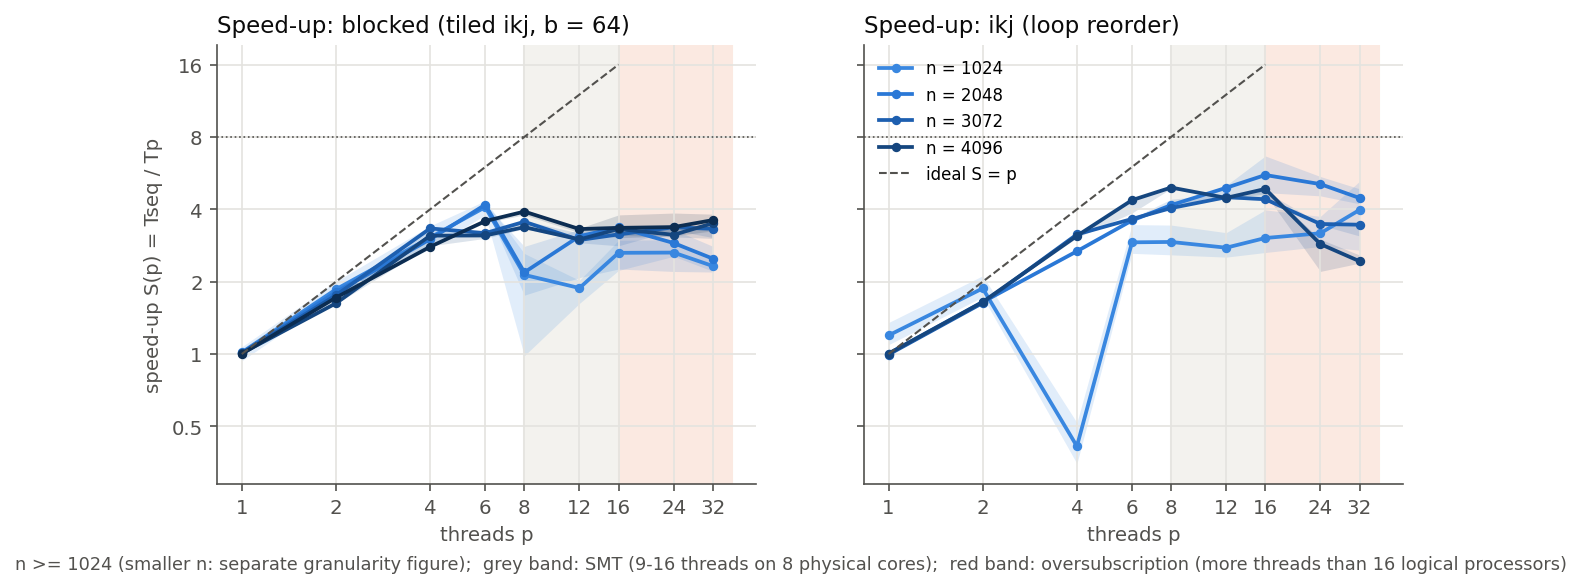
\includegraphics[width=0.84\linewidth]{../results/figures/fig_speedup.png}
\caption{Speed-up against threads for $n\ge1024$. The shaded band is the quartile range of $S$,
the dashed line is $S=p$ and the dotted line is the core count. Grey band: 9--16 threads
share the 8 cores through SMT. Red band: more threads than logical processors.}
\label{fig:speedup}
\end{figure}

\concept{One thread: the cost of the parallel version}
Table~\ref{tab:overhead} compares the sequential kernel with the parallel kernel run with one
thread. For $n\ge2048$ the two differ by at most 1.2\,\%, in both directions. This is less
than the difference between two processes measuring the same configuration
(Section~\ref{sec:repeat}), so no overhead from the OpenMP constructs is measurable there. For
$n\le1024$ the ratio varies from 0.84 to 1.10, within the sample-to-sample variation. For
example, the five samples of \texttt{ikj\_seq} at $n=1024$ range from 213 to 315\,ms, and the
parallel median with one thread (211\,ms) equals the fastest of them.

\begin{table}[H]
\centering
\caption{Sequential baseline against the parallel kernel with $p=1$ (median times).
Ratio $=T_{p=1}/T_\text{seq}$; values above 1 would be parallel overhead.}
\label{tab:overhead}
\small\OverheadTable
\end{table}

\concept{Blocked kernel}
For $n\ge1024$ the speed-up is 1.6--1.9 with 2 threads and 2.8--3.3 with 4 (efficiency
0.70--0.83). It then flattens: the best median speed-up is 4.09 and 4.18 at $p=6$ ($n=1024$,
2048) and 3.55, 3.37 and 3.91 at $p=8$ ($n=3072$, 4096, 6144), with efficiency 0.42--0.70.
From 8 to 16 threads, where SMT siblings are added, the speed-up does not grow at any size
(for example 3.91 to 3.35 at $n=6144$). Throughput peaks at 44.7\,GFLOP/s ($n=2048$, $p=6$)
and 40.9\,GFLOP/s ($n=6144$, $p=8$), against 10.5--10.8\,GFLOP/s sequentially
(Figure~\ref{fig:throughput}). At $n=1024$ and 2048, $p=8$ is \emph{slower} than $p=6$, with
an IQR of 45--128\,\%; Section~\ref{sec:repeat} examines these runs.

\concept{i-k-j kernel}
Sequentially, i-k-j matches blocking up to $n=512$ (11.5\,GFLOP/s). It falls to 5.0--5.2\,GFLOP/s
from $n=2048$ on, where $B$ (32\,MB and more) no longer fits in the 16\,MB L3 cache. In
parallel it scales \emph{further} than blocking: for $n\ge2048$ the speed-up reaches 4.05--4.93
at $p=8$ and 5.56 at $p=16$ ($n=2048$), so SMT adds 9--34\,\% at $n=2048$ and 3072 and nothing
at 4096. Its absolute throughput still stays below that of the blocked kernel: at most
28.6\,GFLOP/s.

\begin{figure}[H]
\centering
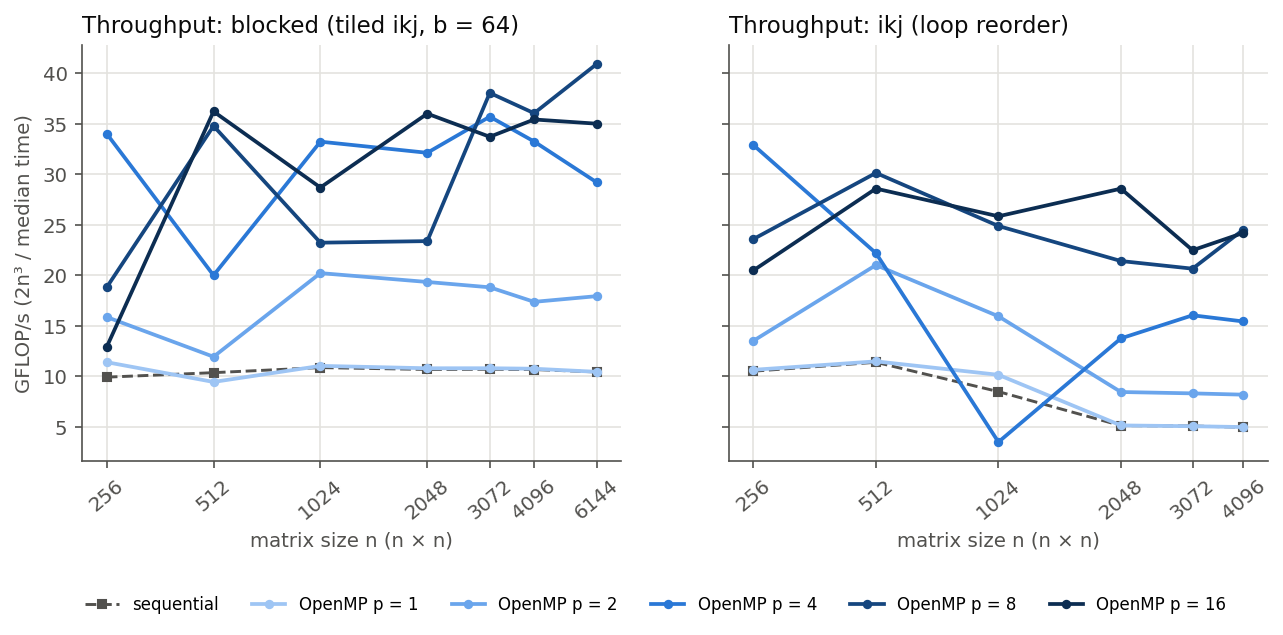
\includegraphics[width=0.84\linewidth]{../results/figures/fig_throughput.png}
\caption{Throughput ($2n^3$ / median time) against $n$ for the sequential baseline and for
$p=1$, 2, 4, 8, 16. The dips of individual lines (e.g.\ i-k-j, $p=4$, $n=1024$) are single
runs disturbed by background activity (Section~\ref{sec:repeat}).}
\label{fig:throughput}
\end{figure}

\concept{Oversubscription}
For the blocked kernel, 24 and 32 threads give times within $\pm$10\,\% of 16 threads for
$n\ge3072$. For i-k-j they are clearly slower when $B$ does not fit in L3. At $n=4096$ the
median time grows from 5.68\,s ($p=16$) to 9.63\,s ($p=24$) and 11.35\,s ($p=32$), which is up
to $2.0\times$ slower and less than half the efficiency. At $n=3072$ the time grows from
2.58\,s to 3.27--3.29\,s.

\concept{Small matrices}
At $n=256$ (3.4\,ms sequentially) and $n=512$ (26\,ms), both kernels reach speed-ups of only about 3--5,
and the curves are irregular. For the blocked kernel the static schedule shares
$\lceil n/64\rceil$ row tiles, which is 4 at $n=256$ and 8 at $n=512$. The best speed-up at
$n=256$, 3.42, is reached exactly at $p=4$; with more threads some of them get no tile but
still join the region and its barrier. At $n=256$ and $p=12$ the time rose to 13.7\,ms, four
times the sequential time (Figure~\ref{fig:granularity}).

\begin{figure}[H]
\centering
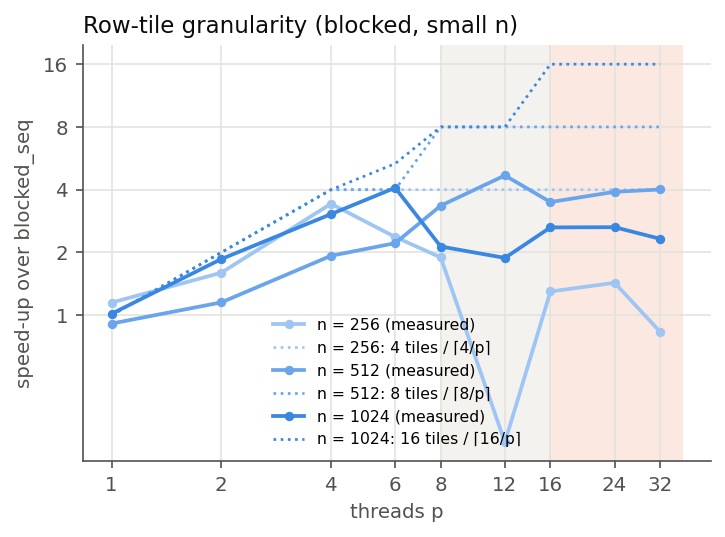
\includegraphics[width=0.5\linewidth]{../results/figures/fig_granularity.png}
\caption{Blocked kernel at small $n$: measured speed-up (solid) and the load-balance bound of
the static schedule, $\text{tiles}/\lceil\text{tiles}/p\rceil$ (dotted).}
\label{fig:granularity}
\end{figure}

\subsection{Variability and repeatability}\label{sec:repeat}
Some configurations of the main study were measured again, in separate processes, by the
placement and vectorisation experiments (same kernel, $n=2048$, SSE2 build, \texttt{spread}).
Table~\ref{tab:repeat} (Appendix~\ref{app:tables}) compares the three medians. With 1 or 2 threads they agree within 2\,\%
for i-k-j and 15\,\% for blocking. With 8 threads, the blocked kernel took 734, 444 and
507\,ms in the three processes (max/min 1.66), and within the scaling run the five samples
ranged from 0.44 to 1.95\,s. In contrast, the blocked kernel with $p=6$ had an IQR below 3\,\%
at every $n\ge2048$. The i-k-j kernel is much less affected (max/min $\le1.09$ up to $p=8$).
The speed-up tables are computed from the scaling run only. Where a value is clearly below its
neighbours, as for blocked at $p=8$, $n=1024$/2048 and i-k-j at $p=4$, $n=1024$, the IQR or this
table shows it to be a disturbed run, not a property of the kernel.


\concept{Follow-up: all $p=8$ configurations repeated with 15 repetitions}
The follow-up ran on 13 November 2026 from 08:22 to 08:29 (UTC), on AC power, with the same
binaries, inputs and protocol, apart from the number of repetitions. Table~\ref{tab:repeat8}
compares it with the main study. Its speed-ups use the sequential medians of the main study.
\begin{itemize}[leftmargin=1.4em]
  \item \textbf{Spread within a run.} It fell where the main study had been disturbed: for the
        blocked kernel the relative IQR went from 128 to 8\,\% at $n=1024$ and from 45 to
        20\,\% at $n=2048$. With these values, $p=8$ is no longer slower than $p=4$ at these
        sizes, and at $n=1024$ it is close to $p=6$ (3.92 against 4.09).
  \item \textbf{Medians.} The repeated medians were up to 50\,\% shorter, including cases where
        the main run had a small IQR: blocked at $n=3072$ and 4096 was 27 and 23\,\% faster
        (IQR 2--6\,\% in the main run). The speed-up rose to 4.87 and 4.38 (efficiency 0.61 and
        0.55, up to 52\,GFLOP/s). At $n=6144$ the two runs agree within 0.4\,\%, and i-k-j at
        $n=4096$ was 7\,\% slower in the repeat.
\end{itemize}
The repeat therefore confirms that the low $p=8$ values at $n=1024$ and 2048 came from
disturbed runs. It also shows that the state of the machine changes between sessions, through
temperature, power management and background load. The difference between two sessions
($-50$ to $+7\,\%$) is larger than the interquartile range within either of them, so the
$p=8$ speed-ups are reliable only to within about 25\,\%. The other thread counts were
not repeated and may carry a similar session effect.

\begin{table}[H]
\centering
\caption{$p=8$ in the main study (12 Nov., 5 repetitions) and in the follow-up (13 Nov.,
15 repetitions), both against the sequential medians of the main study. Last column: the main
study's speed-up with $p=6$, for comparison (\texttt{results/summary/repeat\_p8.csv}).}
\label{tab:repeat8}
\small\resizebox{\linewidth}{!}{\RepeatEightTable}
\end{table}

\subsection{Memory}
Table~\ref{tab:memory} shows that the peak working set equals the storage of $A$, $B$ and $C$
($24n^2$ bytes) plus about 5\,MB of program and runtime. It does not depend on $p$: from 1 to
32 threads it grows by at most 0.8\,MB (thread stacks and runtime data). The i-k-j kernel has the
same footprint (407.6\,MB at $n=4096$ for $p=1$ and 408.3\,MB for $p=32$).

\begin{table}[H]
\centering
\caption{Peak working set of the blocked kernel and peak number of OS threads of the process.}
\label{tab:memory}
\small\resizebox{\linewidth}{!}{\MemoryTable}
\end{table}

\subsection{Thread placement}\label{sec:place}
Figure~\ref{fig:affinity} and Table~\ref{tab:affinity} (Appendix~\ref{app:tables}) compare the placements at $n=2048$.
With \texttt{compact}, $p=2$ puts both threads on the two SMT siblings of one core. The blocked
kernel then takes 1.77\,s, against 1.02\,s with one thread per core (\texttt{spread}). This
is even slower than the sequential kernel (1.61\,s): two threads that share a core do less
work together than one thread alone. The i-k-j kernel loses only 4\,\% (2.14 against
2.05\,s). At $p=4$ and 8, \texttt{compact} is 39--49\,\% slower than \texttt{spread} for
blocking and 10--13\,\% for i-k-j. With 16 threads every logical
processor is used and the three placements agree within the noise. Without pinning
(\texttt{none}) the times are close to \texttt{spread} with 2 threads and between
\texttt{compact} and \texttt{spread} with 4 and 8 for blocking; for i-k-j with 8 threads the
unpinned run was the fastest (706\,ms against 767\,ms). When the threads were sampled
after the measurements, they ran on only 2--5 distinct cores.

\begin{figure}[H]
\centering
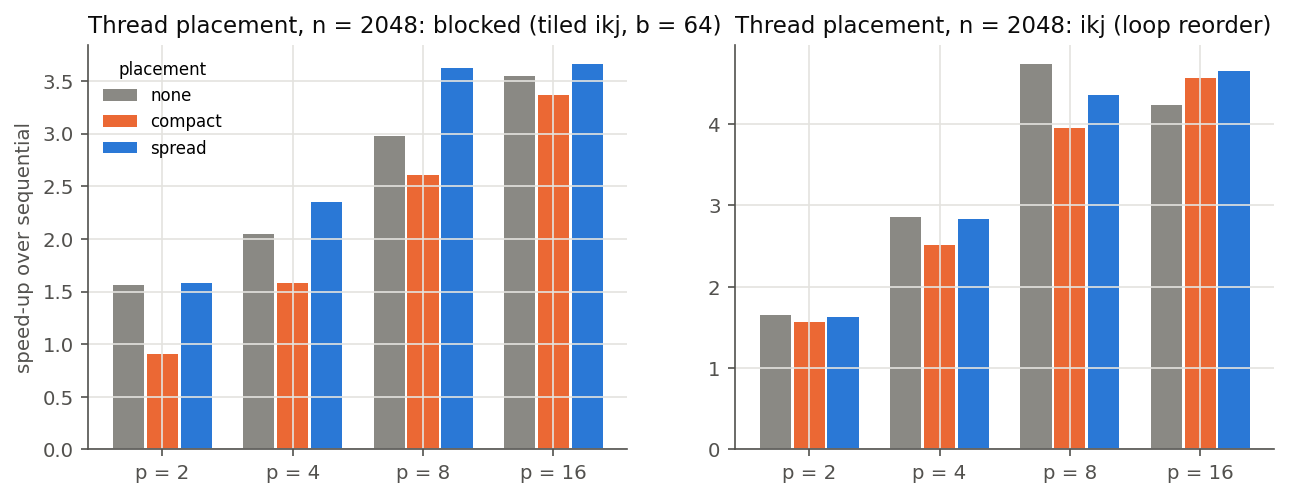
\includegraphics[width=0.84\linewidth]{../results/figures/fig_affinity.png}
\caption{Speed-up over the sequential kernel at $n=2048$ for the three placements.}
\label{fig:affinity}
\end{figure}


\subsection{Clock frequency with more busy cores (supplementary check)}
To explain why even the compute-bound blocked kernel scales sublinearly, a separate short run
after the campaign (\texttt{scripts/frequency\_check.ps1}) sampled the Windows counter
\emph{\% Processor Performance} every 2\,s while \texttt{blocked\_omp} ran at $n=4096$. This
counter gives the effective clock as a percentage of the 2.0\,GHz base clock, and it was
averaged over the logical processors that held the threads (Table~\ref{tab:freq}). The
effective clock falls from 3.5--3.9\,GHz with one or two busy cores to 2.3\,GHz with eight and
2.0\,GHz with sixteen threads. The work per clock cycle and core also falls, from 2.9 to 1.8
floating-point operations. The sampling itself uses processor time (the run with 4 threads was
45\,\% slower than in the campaign), so these numbers show the trend only and are not used in
any other result.

\begin{table}[H]
\centering
\caption{Effective clock of the busy logical processors and throughput of \texttt{blocked\_omp},
$n=4096$, separate run with counter sampling (\texttt{results/frequency\_check.csv}).}
\label{tab:freq}
\small
\begin{tabular}{r r r r r}\toprule
$p$ & effective clock (GHz) & GFLOP/s & FLOP per cycle and core & $S$ predicted by clock alone \\\midrule
1 & 3.47 & 10.0 & 2.89 & 1.00 \\
2 & 3.87 & 16.3 & 2.10 & 2.23 \\
4 & 2.74 & 23.0 & 2.10 & 3.16 \\
8 & 2.28 & 32.8 & 1.80 & 5.26 \\
16 & 2.04 & 35.3 & 2.16\textsuperscript{a} & 4.70\textsuperscript{a} \\
\bottomrule
\multicolumn{5}{l}{\footnotesize\textsuperscript{a} per physical core (8), since the 16 threads share 8 cores.}
\end{tabular}
\end{table}

\subsection{Optional extension: vectorisation}\label{sec:vecres}
\concept{Evidence of vectorisation}
GCC's \texttt{-fopt-info-vec} report (\texttt{results/vectorization\_report.txt}) lists the
inner loop of all four kernels as vectorised, with 16-byte vectors in the default build and
32-byte vectors (unroll factor 4) with \texttt{-mavx2}. It lists no vectorised loop in the
scalar build, and none in \texttt{blocked\_omp\_nosimd}. All three builds give bitwise
identical results (Section~\ref{sec:correct}), so vectorisation changes only the speed.

\concept{Effect, separated from the thread count}
Table~\ref{tab:vec} and Figure~\ref{fig:vec} give the gain of each build over the scalar build
\emph{at the same thread count}. For the blocked kernel, SSE2 gives $1.6\times$ and AVX2
$2.2$--$2.6\times$ with 1 to 4 threads; with 8 and 16 threads the AVX2 gain falls to
$2.06\times$ and $1.77\times$. For i-k-j the gains are smaller ($1.2$--$1.3\times$ and
$1.4$--$1.6\times$) because the kernel waits for memory. Vectorisation and threads combine
but do not multiply fully. The fastest configuration measured, \texttt{blocked\_omp} with AVX2
and 8 threads, took 282\,ms at $n=2048$ (61\,GFLOP/s). That is $9.3\times$ faster than the
scalar sequential kernel, $5.7\times$ faster than the SSE2 sequential baseline, and
$3.7\times$ faster than the AVX2 sequential kernel.

\begin{table}[H]
\centering
\caption{Median time at $n=2048$ for the three builds; gain over the scalar build at the same
$p$; and speed-up of the AVX2 build over the scalar sequential kernel.}
\label{tab:vec}
\small\resizebox{\linewidth}{!}{\VecTable}
\end{table}

\begin{figure}[H]
\centering
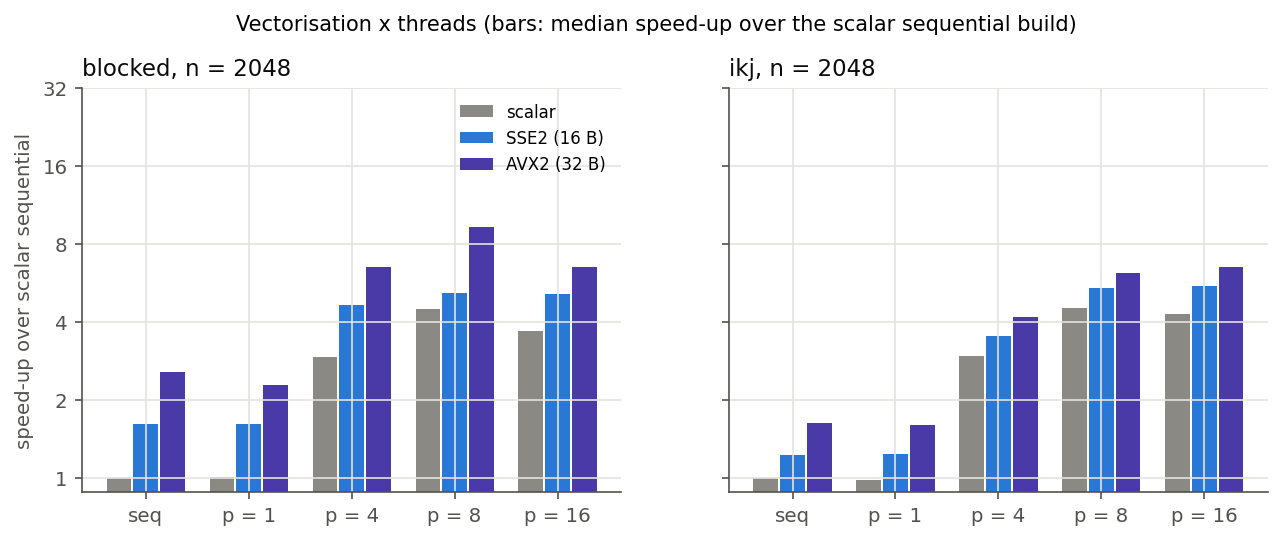
\includegraphics[width=0.84\linewidth]{../results/figures/fig_vectorization.png}
\caption{Speed-up over the scalar sequential kernel at $n=2048$, by build and thread count
(logarithmic scale).}
\label{fig:vec}
\end{figure}

\concept{The \texttt{omp simd} directive}
Table~\ref{tab:simd} (Appendix~\ref{app:tables}) shows that without \texttt{omp simd} the one-thread parallel kernel
takes 2.58\,s at $n=2048$. This is the time of the scalar build (2.61\,s) and $1.62\times$
slower than with the directive, as the vectorisation report predicts. With 16 threads the
directive is again worth $1.5$--$1.6\times$. With 8 threads the variant without it (593\,ms)
falls inside the 444--734\,ms range of the three measurements with it, an instance of the
disturbed $p=8$ runs of Section~\ref{sec:repeat}.


% =====================================================================
\FloatBarrier
\section{Discussion}

\concept{H1 -- the blocked kernel scales almost linearly to 8 cores: rejected}
Its efficiency is 0.70--0.83 at 4 threads but only 0.42--0.49 at 8 for $n\ge3072$ in the main
study, and 0.49--0.61 in the follow-up, against the expected $\ge0.8$. Arithmetic intensity is not the limit. With tile 64 \cite{lam}, the blocked kernel moves
about $24n^3/64$ bytes between cache levels for $2n^3$ operations, so its 40\,GFLOP/s need only
about 8\,GB/s, well within the 51.2\,GB/s of the two DDR4-3200 channels. Two other limits
appear instead.
\begin{itemize}[leftmargin=1.4em]
  \item \textbf{Power-limited clock.} The 7730U is a 15\,W laptop processor. Table~\ref{tab:freq}
        shows the effective clock falling by a factor 1.5 from one busy core to eight, which
        alone caps $S(8)$ at about 5.3. The rest of the gap, 5.3 against the 3.4--4.9 measured,
        matches the fall in work per cycle (2.9 to 1.8 FLOP per cycle and core). That
        fall is consistent with eight cores competing for the shared L3 and memory, which this
        study did not measure directly. Assignment~2's single-core results were therefore
        obtained at a clock that eight cores cannot sustain.
  \item \textbf{Static schedule with every core pinned.} With 8 pinned threads every physical core
        holds one, and \texttt{schedule(static)} fixes each thread's share in advance. Any other
        work, such as an OS service, the benchmark driver sampling memory every 20\,ms or a
        background application, must then interrupt one of them. The barrier at the end of the
        loop waits for that thread, so the whole team waits. This explains the spread at
        $p=8$ (0.44--1.95\,s for the same configuration) and why $p=6$, which leaves two cores
        free, was faster than $p=8$ at $n=1024$ and 2048 and stable (IQR $<3\,\%$) at every
        $n\ge2048$. The follow-up, in a quieter session, brought $p=8$ back to the level of
        $p=6$ at $n=1024$, which supports interference rather than a property of the kernel.
        The i-k-j kernel
        is less affected. A plausible reason is that it is limited by memory, so a short delay
        on one core overlaps with time the others spend waiting for data.
\end{itemize}

\concept{H2 -- SMT adds little, oversubscription adds nothing: supported, with a nuance}
For the compute-bound blocked kernel the second hardware thread of a core is useless or
harmful. From 8 to 16 threads the speed-up does not rise, and two siblings on one core
(\texttt{compact}, $p=2$) are slower than one thread alone. They share the core's vector units
and its 32\,KB L1 cache, into which the $64\times64$ tile of $B$ (32\,KB) alone already fills.
For the memory-bound i-k-j kernel SMT gives 9--34\,\% at $n=2048$ and 3072, because one sibling
can compute while the other waits for memory. This is the case where SMT is expected to help
\cite{hennessy}. Oversubscription never helped. It was neutral for blocking, but up to
$2\times$ slower for i-k-j at $n=4096$. With more threads than logical processors the
operating system time-slices them, a descheduled thread stalls the barrier, and libgomp
reduces its spinning \cite{libgomp}. For i-k-j the extra threads also stream different rows of
$B$ at different times, which removes the shared-L3 effect described next.

\concept{H3 -- i-k-j saturates on memory bandwidth: partly rejected}
The sequential i-k-j kernel does become memory-bound once $B$ exceeds the L3 cache: its
throughput halves from 11.5 to 5.1\,GFLOP/s. But its speed-up was \emph{higher} than that of
blocking (up to 5.56 against 4.18), the opposite of the hypothesis, for two reasons.
\begin{itemize}[leftmargin=1.4em]
  \item One core cannot use the full bandwidth of the memory system: it is limited by how many
        cache misses it can keep in flight. So the sequential baseline is slow, and several
        cores add bandwidth.
  \item The threads do not each fetch their own copy of $B$. At 24.5\,GFLOP/s with $p=8$
        ($n=4096$), fetching all of $B$ from DRAM for every row of $C$ would need
        $8n^3/T=98$\,GB/s, almost twice the 51.2\,GB/s peak. All threads walk through $B$ in the
        same $k$ order at roughly the same pace, so a row of $B$ brought into the shared L3 by
        one thread is reused by the others.
\end{itemize}
The speed-up of i-k-j is high because its baseline is poor. In absolute terms it is still the
worse kernel: its best result, 28.6\,GFLOP/s, is below what the blocked kernel reaches with
4 threads. The lesson of Assignment~2, which is to optimise memory access first, still holds
in parallel. A higher speed-up does not mean a faster program.

\concept{H4 -- small matrices are limited by overheads and granularity: supported}
With a static schedule over $\lceil n/64\rceil$ row tiles the blocked kernel cannot use more
than 4 threads at $n=256$ or 8 at $n=512$. The measurements follow this bound: the best value
at $n=256$ is exactly at $p=4$, and extra threads only add synchronisation. At these sizes a
multiplication takes 1--26\,ms, so a few milliseconds of disturbance or barrier waiting
dominate. The very large IQRs in Table~\ref{tab:time} at $n\le1024$ reflect this. Parallel
execution therefore pays off from about $n=512$, and only with as many threads as there are
tiles or rows to share.

\concept{H5 -- memory does not grow with $p$: supported}
The threads share $A$, $B$ and $C$ and allocate nothing, so the peak working set is the
$24n^2$ model plus a constant 5\,MB at every $p$. Each extra thread adds only about 25\,KB to the
working set, for its stack and runtime bookkeeping (0.8\,MB for 31 extra threads). The only memory cost of parallelism here is
therefore the operating-system threads ($p+3$), not data.

\concept{Superlinear speed-up}
No configuration with $p\ge2$ was superlinear; the highest efficiency was 0.94 (i-k-j,
$n=1024$, $p=2$). Efficiencies above 1 appear only at $p=1$ and small $n$: 1.15 for blocked at
$n=256$ and 1.20 for i-k-j at $n=1024$. Both come from variability of the sequential samples
(IQR 15--18\,\%), not from a real effect: the parallel one-thread median is within 5\,\% of
the fastest sequential sample (211 against 213\,ms; 2.94 against 3.09\,ms). A real superlinear speed-up would need each thread's working set to fit in
a cache that the sequential run overflows. Here the large shared operand $B$ does not shrink
when divided among threads, so this was not expected.

\concept{When does parallel execution help?}
On this machine parallel execution helped from $n\approx512$ upward. The useful range was
$p=4$--8 threads, one per physical core, pinned \texttt{spread}. Leaving one or two cores free
($p=6$) gave nearly the same speed with far less variability. SMT siblings helped only the
memory-bound kernel, and more threads than logical processors never helped. Thread placement
mattered as much as thread count. Putting two threads on one core (\texttt{compact}) made the
blocked kernel slower than not parallelising at all, so placement must be recorded in any
speed-up claim. The single-thread overhead of the OpenMP version was not measurable for
$n\ge2048$, so the parallel code can replace the sequential one without loss.

\concept{Vectorisation and threads}
Vectorisation is the cheaper speed-up: AVX2 gave the blocked kernel $2.6\times$ on one core
without using any other core, more than the $1.8\times$ from a second thread. The two do not
multiply fully. With 8 or 16 threads, and for the memory-bound i-k-j kernel, the AVX2 gain
shrinks to $1.4$--$2.1\times$, because the work moves toward the memory system that vector
width does not speed up. The \texttt{omp simd} finding is a methodological one. Without it,
the parallel kernel would have been compared in scalar form against a vectorised baseline, and
every speed-up in this report would have been $1.6\times$ too small at one thread. Compiler
reports, not only timings, are needed to make the comparison fair.

\concept{Limitations}
\begin{itemize}[leftmargin=1.4em]
  \item One laptop under a 15\,W power limit, in the ``Balanced'' power plan and with normal
        background activity. A desktop or server processor with a higher power budget, or more
        memory channels, would scale further. Absolute numbers apply only to this machine.
  \item Only own C kernels were parallelised. A tuned BLAS library uses register blocking and
        packing \cite{goto}, reaches several times the single-core throughput measured here and
        may scale differently; it was deliberately left out so that the parallel and sequential
        versions run exactly the same loop nest.
  \item Five repetitions per configuration were enough when the machine was quiet, but not at
        $p=8$. Fifteen repetitions in the follow-up reduced the spread within a run, but not
        the difference between sessions (up to 50\,\%). Only the $p=8$ cases were repeated, so
        a session effect on the other thread counts cannot be excluded. Repeating the whole
        campaign in several sessions, alternating the configurations, would be needed to
        measure it.
  \item Only \texttt{schedule(static)} was tested. A \texttt{dynamic} or \texttt{guided}
        schedule over smaller chunks might absorb the delays of interrupted threads at
        $p=8$. Testing it is the obvious next step.
  \item The clock measurement is a separate, perturbing run with a coarse counter. It supports
        the explanation of the scaling limit qualitatively but does not separate clock, cache
        and memory effects. Hardware performance counters were not available.
  \item \texttt{OMP\_PLACES} could not be used with libgomp on Windows, so pinning is custom
        code. It was verified after the measurements, not during them.
\end{itemize}

% =====================================================================
\section{Conclusions}

\begin{itemize}[leftmargin=1.4em]
  \item \textbf{Correctness.} Sharing the outer loop of the Assignment~2 kernels with
        \texttt{omp for schedule(static)} is safe without locks. It reproduced the sequential
        result bit for bit in all 203 runs (190 + 13 follow-up), at 1 to 32 threads, in every placement and in every
        build.
  \item \textbf{One-thread overhead.} Negligible: within 1.2\,\% of the sequential kernel for
        $n\ge2048$. This holds only once the parallel loop is vectorised like the sequential
        one (\texttt{omp simd}). Without that, the parallel kernel was $1.6\times$ slower with
        one thread.
  \item \textbf{Scaling.} The best median speed-ups were 3.4--4.2 for the blocked kernel
        (efficiency 0.42--0.70, at 6--8 threads) and 4.5--5.6 for i-k-j ($n\ge2048$). The peak
        was 44.7\,GFLOP/s, against 10.8\,GFLOP/s sequentially. The $p=8$ follow-up gave up to
        4.9 (52\,GFLOP/s), and the differences between sessions were as large as 50\,\%, so
        these values describe a range of about $4$--$5\times$ rather than a single
        number. The limits are the 15\,W power
        budget, which lowers the clock as cores are added, shared cache and memory, and the
        sensitivity of a pinned static schedule to any interruption when all cores are
        busy.
  \item \textbf{SMT, oversubscription and placement.} SMT helped only the memory-bound kernel
        (up to $+34\,\%$). Oversubscription never helped and made i-k-j up to $2\times$ slower.
        Two threads on one core made the blocked kernel slower than sequential. The right
        configuration is one thread per physical core, spread, possibly leaving one or two
        cores free.
  \item \textbf{Granularity and memory.} Small matrices are bounded by the number of row tiles
        ($S\le4$ at $n=256$). Memory does not grow with $p$: less than 1\,MB from 1 to 32
        threads.
  \item \textbf{Vectorisation (extension).} AVX2 made each kernel 1.4--2.6 times faster at the
        same thread count. Combined with 8 threads it reached 61\,GFLOP/s, $9.3\times$ the
        scalar sequential kernel. On this laptop, vector width gives more per core than SMT,
        and more than adding a second core ($2.6\times$ against $1.8\times$).
\end{itemize}
The research question therefore has a qualified answer. On a power-limited 8-core laptop,
threads speed up a well-optimised dense multiplication by about $4\times$, not $8\times$, and
only for $n\gtrsim512$. The best thread count is the number of physical cores or slightly
fewer, not the number of logical processors.

\concept{What remains unresolved}
The study does not separate how much of the gap between the clock-predicted speed-up (5.3 at
$p=8$) and the measured one (3.4) is due to shared-cache or memory contention and how much to
interference; hardware counters would be needed. Whether a \texttt{dynamic} schedule removes the
instability at $p=8$, and whether the conclusions hold on a processor without a 15\,W power
limit, were not tested.

% =====================================================================
\section*{Reproducibility materials}
Repository: \url{\RepoURL}. It contains the source code (\texttt{c/}; the sequential kernel bodies
are copied unchanged from Assignment~2, \url{\ATwoURL}, and the self-test reference from
Assignment~1, \url{\AOneURL}), the configuration (\texttt{config/benchmark\_config.json}), the
input generator with the SHA-256 of every input (\texttt{scripts/generate\_inputs.py}), the
build, benchmark, validation and analysis scripts, a one-command campaign script
(\texttt{scripts/run\_campaign.sh}), all raw measurements (\texttt{results/raw/}), and a README
with exact commands and dependency versions.

\section*{Use of generative AI}
Claude Opus (Anthropic), used through Claude Code, assisted with: writing and debugging the C
program and the Python scripts (input generation, benchmark driver, validation, analysis and
figures); diagnosing the code-generation differences described in the methodology; running the
measurement campaign on the author's machine; and drafting and revising the text of this report.
The author defined the study, reviewed the code and checked every number in the report against
the raw data in the repository. Generated content was not used as evidence: all results come
from executing the code, and all references were checked to exist.

% =====================================================================
\begin{thebibliography}{99}\small\sloppy
\setlength{\itemsep}{1pt}
\bibitem{openmp} OpenMP Architecture Review Board, ``OpenMP Application Programming Interface, Version 5.1,'' Nov. 2020. [Online]. Available: \url{https://www.openmp.org/specifications/}
\bibitem{chapman} B.~Chapman, G.~Jost, and R.~van~der~Pas, \emph{Using OpenMP: Portable Shared Memory Parallel Programming}. Cambridge, MA, USA: MIT Press, 2008.
\bibitem{amdahl} G.~M. Amdahl, ``Validity of the single processor approach to achieving large scale computing capabilities,'' in \emph{Proc. AFIPS Spring Joint Computer Conf.}, 1967, pp.~483--485.
\bibitem{roofline} S.~Williams, A.~Waterman, and D.~Patterson, ``Roofline: An insightful visual performance model for multicore architectures,'' \emph{Commun. ACM}, vol.~52, no.~4, pp.~65--76, 2009.
\bibitem{hennessy} J.~L. Hennessy and D.~A. Patterson, \emph{Computer Architecture: A Quantitative Approach}, 6th ed. Cambridge, MA, USA: Morgan Kaufmann, 2019.
\bibitem{libgomp} GNU Project, ``GNU Offloading and Multi Processing Runtime Library (libgomp) manual,'' 2026. [Online]. Available: \url{https://gcc.gnu.org/onlinedocs/libgomp/}
\bibitem{msaffinity} Microsoft, ``SetThreadAffinityMask function (winbase.h)'' and ``GetLogicalProcessorInformationEx function (sysinfoapi.h),'' Microsoft Learn, 2026. [Online]. Available: \url{https://learn.microsoft.com/en-us/windows/win32/api/winbase/nf-winbase-setthreadaffinitymask}
\bibitem{gcc12} GNU Project, ``GCC 12 Release Series: Changes, New Features, and Fixes,'' 2022. [Online]. Available: \url{https://gcc.gnu.org/gcc-12/changes.html}
\bibitem{lam} M.~S. Lam, E.~E. Rothberg, and M.~E. Wolf, ``The cache performance and optimizations of blocked algorithms,'' in \emph{Proc. ASPLOS-IV}, 1991, pp.~63--74.
\bibitem{goto} K.~Goto and R.~A. van~de~Geijn, ``Anatomy of high-performance matrix multiplication,'' \emph{ACM Trans. Math. Softw.}, vol.~34, no.~3, art.~12, 2008.
\bibitem{higham} N.~J. Higham, \emph{Accuracy and Stability of Numerical Algorithms}, 2nd ed. Philadelphia, PA, USA: SIAM, 2002.
\bibitem{amd} Advanced Micro Devices, ``Software Optimization Guide for AMD Family 19h Processors,'' Pub. no. 56665, 2020.
\bibitem{psutil} G.~Rodola, ``psutil documentation,'' 2026. [Online]. Available: \url{https://psutil.readthedocs.io/}
\end{thebibliography}

% =====================================================================
\clearpage
\appendix
\section{Additional tables}\label{app:tables}
These tables give the detail behind Sections~\ref{sec:repeat}, \ref{sec:place} and \ref{sec:vecres}; all values come from \texttt{results/summary/summary.csv}.

\begin{table}[H]
\centering
\caption{Median time per multiplication (relative IQR in \%, small type). Main study,
placement \texttt{spread}, SSE2 build. The sequential column is the baseline $T_\text{seq}$.}
\label{tab:time}
\small
\textbf{(a) blocked} (\texttt{blocked\_seq} / \texttt{blocked\_omp})\\[2pt]
\resizebox{\linewidth}{!}{\BlockedTimeTable}\\[6pt]
\textbf{(b) i-k-j} (\texttt{ikj\_seq} / \texttt{ikj\_omp})\\[2pt]
\resizebox{\linewidth}{!}{\IkjTimeTable}
\end{table}

\begin{table}[H]
\centering
\caption{The same configuration ($n=2048$, SSE2, \texttt{spread}) measured by three
experiments in separate processes: median time (relative IQR in \%).}
\label{tab:repeat}
\small\RepeatTable
\end{table}

\begin{table}[H]
\centering
\caption{Median time at $n=2048$ by placement (relative IQR in \%). Last column: distinct
physical cores used by the threads of the unpinned run, sampled after the measurements.}
\label{tab:affinity}
\small\AffinityTable
\end{table}

\begin{table}[H]
\centering
\caption{Blocked parallel kernel with and without \texttt{omp simd} (median time). ``With''
is taken from the scaling run and, at $n=2048$, also from the vectorisation run. Ratio
$=$ without / scaling run.}
\label{tab:simd}
\small\SimdTable
\end{table}

\end{document}
